\documentclass[12pt]{report}	%worth trying refman, memoir classes (memoir manual is recommended read)
\usepackage[usenames]{color}
\usepackage{titlesec}
\setcounter{secnumdepth}{3}
\setcounter{tocdepth}{3}
\usepackage[utf8]{inputenc}
\usepackage{parskip}
\usepackage{setspace}
\titleformat{\chapter}[block]
  {\normalfont\huge\bfseries}{\thechapter.}{0.5em}{\Huge}
% \titlespacing*{\chapter}{0pt}{-19pt}{0pt}
\usepackage[ampersand]{easylist}
\usepackage{graphicx}
\graphicspath{ {data/} }
\usepackage{tabularx}
\usepackage{longtable}
\usepackage{xtab}
\usepackage[breaklinks=true]{hyperref}
\hypersetup{pdfpagemode=UseOutlines}
\usepackage{fdsymbol}
\usepackage{bm}
\usepackage[toc,page]{appendix}
\usepackage{alltt}
\usepackage{marvosym}
\newcommand*{\TakeFourierOrnament}[1]{{%
\fontencoding{U}\fontfamily{futs}\selectfont\char#1}}
\newcommand*{\danger}{\TakeFourierOrnament{66}}


\begin{document}
\title{HoustonTracker 2 Manual}
%\author{utz/irrlicht project}
\date{\today}
\maketitle
\pagenumbering{roman}
\tableofcontents

\renewcommand{\abstractname}{Note}
\begin{abstract}
This manual applies to the latest beta version of HoustonTracker 2. To see the online manual for the latest stable release, visit \href{http://irrlichtproject.de/houston/manual.html}{\nolinkurl{http://irrlichtproject.de/houston/manual.html}}.
\end{abstract}

\pagenumbering{arabic}
\chapter{About}

\section{What is HoustonTracker 2?}
HoustonTracker 2 is a software sequencer that enables you to create music on Texas Instruments graphing calculators. It uses the machines' communication port to output multi-channel 1-bit music. Its interface is inspired by popular trackers such as LSDJ, Famitracker, and Milkytracker.

HT2 supports several models of the Z80-based line of TI calculators. It is mainly targetted at older, obsolete models like the TI-82, but also works on newer machines up to and including the TI-84 Plus SE. For a complete list of supported models, see \autoref{sec:supportedmodels}.

\section{Features}
\begin{easylist}[itemize]
\ListProperties(Style2*=$\circ$ )
& 3 tone channels
& 1 non-interrupting drum channel
& up to 128 note patterns
& up to 64 drum/fx patterns
& sequence length up to 255 pattern rows
& 16-bit frequency precision
& 10-bit speed precision, can be configured per step
& various effects, including:
&& L/C/R stereo hard-panning for tone and drum channels
&& advanced duty cycle modulation
&& noise and glitch effects
&& pitch slides
& 2 user definable samples
& up to 8 savestates
& edit during playback
\end{easylist}


\section{Supported Calculator Models}
\label{sec:supportedmodels}
The following table gives an overview over which TI calculator models are supported by HoustonTracker 2. If your calculator isn't listed in the table, chances are HT2 doesn't support it. 
\\ \\ 
\scalebox{0.8}{
\begin{tabular}{l c c c c c}
  \textbf{model} & \textbf{ROM version} & \textbf{shell} & \textbf{HT2 build} & \textbf{status} \\
  \hline
  TI-73, 73 Explorer & all & mallard & \textendash & \textcolor{blue}{planned} \\
  TI-76.fr & all & Ion & ht2.83p & \textcolor{blue}{untested} \\
  TI-81 & \textendash & \textendash & \textendash & \textcolor{red}{not supported} \\
  TI-82	& \textless 16.0 & \textendash & \textendash & \textcolor{blue}{planned} \\
  TI-82	& 16.0-19.0 & CrASH 1.6 & ht2.82p & \textcolor{green}{supported} \\
  TI-82 Parcus & 19.006	& CrASH\_19006 & ht2p.82p & \textcolor{green}{supported} \\
  TI-82 Advanced & \textendash & \textendash & \textendash & \textcolor{red}{not supported} \\
  TI-82 Stats, Stats.fr	& all & Ion & ht2.83p & \textcolor{green}{supported} \\
  TI-82 Plus & all & DoorsCS & ht2(s).8xp & \textcolor{green}{supported} \\
  TI-83 (all versions) & all & Ion & ht2.83p & \textcolor{green}{supported} \\
  TI-83 Plus (all versions) & all & DoorsCS & ht2(s).8xp & \textcolor{green}{supported} \\
  TI-84 Plus/Plus SE & all & DoorsCS & ht2(s).8xp & \textcolor{green}{supported} \\
  TI-84 Plus CSE/CE & \textendash & \textendash & \textendash & \textcolor{red}{not supported} \\
  TI-85, 86 & \textendash & \textendash & \textendash & \textcolor{red}{not supported} \\
  TI-89, 92, 92+, V200 & \textendash & \textendash & \textendash & \textcolor{red}{not supported} \\
\end{tabular}
}
\\ \\ 
Models marked as "not supported" have differences in architecture that would require a major rewrite of HT2. There are no plans to support these models in the near future, especially not the 84+ Color models.


\section{License}
HoustonTracker 2 is free, open source software. It is released under a "Revised" BSD-License. This means you're basically free to use, modify, and redistribute this software both in binary as well as source form, as long as you don't pretend that I endorse what you're doing, or try to hold me responsible for any damage done.

The full license terms are as follows: \newline

{\scriptsize
\begin{verbatim}
Copyright (c) 2015-2016, utz/irrlicht project
All rights reserved.

Redistribution and use in source and binary forms, with or without
modification, are permitted provided that the following conditions are met:
   * Redistributions of source code must retain the above copyright
     notice, this list of conditions and the following disclaimer.
   * Redistributions in binary form must reproduce the above copyright
     notice, this list of conditions and the following disclaimer in the
     documentation and/or other materials provided with the distribution.
   * Neither the name of IRRLICHT PROJECT nor the
     names of its contributors may be used to endorse or promote products
     derived from this software without specific prior written permission.

THIS SOFTWARE IS PROVIDED BY THE COPYRIGHT HOLDERS AND CONTRIBUTORS "AS IS" AND
ANY EXPRESS OR IMPLIED WARRANTIES, INCLUDING, BUT NOT LIMITED TO, THE IMPLIED
WARRANTIES OF MERCHANTABILITY AND FITNESS FOR A PARTICULAR PURPOSE ARE
DISCLAIMED. IN NO EVENT SHALL THE COPYRIGHT HOLDER BE LIABLE FOR ANY
DIRECT, INDIRECT, INCIDENTAL, SPECIAL, EXEMPLARY, OR CONSEQUENTIAL DAMAGES
(INCLUDING, BUT NOT LIMITED TO, PROCUREMENT OF SUBSTITUTE GOODS OR SERVICES;
LOSS OF USE, DATA, OR PROFITS; OR BUSINESS INTERRUPTION) HOWEVER CAUSED AND
ON ANY THEORY OF LIABILITY, WHETHER IN CONTRACT, STRICT LIABILITY, OR TORT
(INCLUDING NEGLIGENCE OR OTHERWISE) ARISING IN ANY WAY OUT OF THE USE OF THIS
SOFTWARE, EVEN IF ADVISED OF THE POSSIBILITY OF SUCH DAMAGE. 
\end{verbatim}
}



\chapter{Conventions, Terms, and Definitions}

The following section outlines some basic terms and conventions used in HoustonTracker 2, and in this documentation.

\subparagraph{Keypress conventions}
In this document, keypresses are denoted in bold font, surrounded by square brackets. All keypresses in HT2 are sequential, meaning you never need to press more than one key at the same time.

For example, \textbf{[ALPHA], [GRAPH], [ENTER]} means you should first press the ALPHA key, then the GRAPH key, and finally the ENTER key.

\subparagraph{Hexadecimal notation}
Hexadecimal numbers in this document are prefixed with 0x. So 0x20 = \$20 = 20h = 32 decimal.
All numbers in the HoustonTracker 2 user interface itself are hexadecimal, therefore no prefix is used there.

\newpage
\subparagraph{Terminology} ~\\
 
\begin{tabularx}{\textwidth}{r X}
\textbf{bit} & This humble binary digit is at the core of HT2's inner workings. It can take a value of 0 (off) or 1 (on). \\
\textbf{byte} & Not related to chewing by any means, the byte is an 8-bit number. It can take any value from 0x00 (decimal 0) to 0xFF (255). \\
\textbf{duty cycle} & The relative amount of time each of the two half-periods of a square wave will consume. \\
\textbf{hi-byte} & The left two hexadecimal digits, aka most significant byte of a word. \\
\textbf{lo-byte} & The right two hexadecimal digits, aka least significant byte of a word. \\
\textbf{nibble} & A single hexadecimal digit. It consists of 4 bits, and can therefore take a value from 0x0 to 0xF (15). \\
\textbf{pattern} & A list of events that makes up a part of a tune. These can be notes, drum triggers, or effect commands. All patterns in HT2 are 16 steps long. \\
\textbf{pitch} &The (perceived) frequency of a tone. \\
\textbf{shell} &A program that facilitates the execution of machine language programs on your TI calculator, among other things. You'll need to install one in order to run HT2. \\
\textbf{song sequence} & A matrix containing the order of patterns. Think of it as a storyboard, or the song's masterplan. \\
\textbf{word} & A 16-bit value. Equivalent to two bytes, or four hexadecimal digits. \\
\end{tabularx}

% \begin{xtabular}{r p{0.8\textwidth}}
% \textbf{bit} & This humble binary digit is at the core of HT2's inner workings. It can take a value of 0 (off) or 1 (on). \\
% \textbf{byte} & Not related to chewing by any means, the byte is an 8-bit number. It can take any value from 0x00 (decimal 0) to 0xFF (255). \\
% \textbf{duty cycle} & The relative amount of time each of the two half-periods of a square wave will consume. \\
% \textbf{hi-byte} & The left two hexadecimal digits, aka most significant byte of a word. \\
% \textbf{lo-byte} & The right two hexadecimal digits, aka least significant byte of a word. \\
% \textbf{nibble} & A single hexadecimal digit. It consists of 4 bits, and can therefore take a value from 0x0 to 0xF (15). \\
% \textbf{pattern} & A list of events that makes up a part of a tune. These can be notes, drum triggers, or effect commands. All patterns in HT2 are 16 steps long. \\
% \textbf{pitch} &The (perceived) frequency of a tone. \\
% \textbf{shell} &A program that facilitates the execution of machine language programs on your TI calculator, among other things. You'll need to install one in order to run HT2. \\
% \textbf{song sequence} & A matrix containing the order of patterns. Think of it as a storyboard, or the song's masterplan. \\
% \textbf{word} & A 16-bit value. Equivalent to two bytes, or four hexadecimal digits. \\
% \end{xtabular}


\chapter{Setup}
\section{Requirements}

\subparagraph{Hardware} ~\\
\begin{easylist}[itemize]
& a TI graphing calculator (see \nameref{sec:supportedmodels})
& a suitable PC\textless-\textgreater Calc link cable, e.g. \href{https://education.ti.com/en/us/products/computer_software/connectivity-software/silver-usb-cable-for-windows-mac/features/features-summary}{TI SilverLink} (recommended), \href{http://guide.alibaba.com/shop/texas-instruments-instruments-ti-graphlink-serial-cable-for-windows_10284857.html}{TI GraphLink}, homemade \href{http://www.ticalc.org/hardware/cables/parallel.html}{parallel} or \href{http://www.ticalc.org/hardware/cables/serial.html}{serial} cable for data transfers
& a 2.5mm (micro-)jack adapter/cable for sound
\end{easylist}
\begin{tabularx}{\textwidth}{m{0.075\textwidth} X}
\textcolor{black}{\newline\Huge\PointingHand} & You can use a cheap calc-to-calc link cable to make your own 2.5mm adapter. \\
\Huge{\textcolor{red}{\newline\danger}} & The plastic base of many adapters is too thick to fit into TI's extra narrow socket. If that's the case, you need to carefully scrape off some plastic from the base of the jack until it fits. \\
\end{tabularx}

\subparagraph{Software} ~\\
In addition to the HT2 executable, you will also need to obtain:
\\ 
\begin{easylist}[itemize]
& TI linking software for exchanging data between your PC and your calc (\href{http://lpg.ticalc.org/prj_tilp/}{TiLP} is strongly recommended, though it can be somewhat tricky to install. Check the \nameref{sec:troubleshoot} guide if you run into problems.)
& a so-called "shell" for your calculator. The following table lists the recommended shells for each model. Other shells may work, but haven't been tested. 
\end{easylist} ~\\
\begin{tabularx}{\textwidth}{l X}
\textbf{model} & \textbf{shell} \\
\hline
TI-82 & \href{http://www.ticalc.org/pub/82/asm/shells/crashsdk.zip}{CrASH 1.6} \\
TI-82 Parcus & \href{http://www.ticalc.org/pub/82/asm/shells/crash19006.zip}{CrASH\_19.006} \\
TI-83, TI-82Stats & \href{http://www.ticalc.org/pub/83/asm/shells/ion16u.zip}{Ion 1.6U} \\
TI-83 Plus, TI-84 Plus & \href{http://dcs.cemetech.net/}{Doors CS 7} \\
\end{tabularx} ~\\

\begin{tabularx}{\textwidth}{m{0.075\textwidth} X}
\Huge{\textcolor{red}{\danger}} & HT2 is not compatible with MirageOS. \\
\Huge{\textcolor{black}{\newline\PointingHand}} & If you don't own a TI calc, you can run HT2 on an emulator. The beta version of tilem2 is recommended. A Win32 installer can be found \href{http://tilem.sourceforge.net/beta/tilem-2.1-beta-20161022.exe}{here}, *nix users can obtain the development version via \emph{svn checkout https://tilem.svn.sourceforge.net/svnroot/tilem/trunk tilem}. You need to have TiLP installed in any case. \\
\end{tabularx}

\section{Installation}
\begin{tabularx}{\textwidth}{m{0.075\textwidth} X}
\Huge{\textcolor{red}{\newline\danger}} & \textbf{\textcolor{red}{After installing HoustonTracker 2, your calculator will not be able to perform most of its regular tasks until HT2 is removed. Do not install HT2 if you need to use your calculator for regular work, such as in school or university.}} \\
\end{tabularx} ~\\

The following instructions assume that you have TiLP installed on your computer. If you are using another linking program, then you probably know what to do...

\newpage
\subparagraph{Installing on TI82/82 Parcus} ~\\

\begin{easylist}
& If you aren't sure which TI82 version you have, press \textbf{[MODE], [ALPHA], [LN]} to check the ROM version. If it says "19.006", you have a 82 Parcus, else you have a regular 82. Afterwards, press any key except Enter.
& Reset your calculator by pressing \textbf{[2nd], [$\bm{+}$], [3]}.
& Switch off your calculator, and connect it to your computer with a link cable.
& Switch the calculator back on.
& On your computer, open TiLP. Make sure your calculator and link cable settings are correct - if not, press Ctrl+D to reconfigure.
& Put your calculator into transmission mode by pressing \textbf{[2nd], [X,T,$\bm{\Theta}$], [\(\medblacktriangleright\)], [ENTER]}.
& In Tilp, go to "File"-\textgreater"Restore", and select CRASH.82B (regular TI82) resp. CRASH19006.82b (82 Parcus). Doing so will prompt for confirmation on both TiLP and your calc.
& Assuming all went good, you can now put your calc in transmission mode again, and send ("File"-\textgreater"Send Files") ht2.82p (regular) resp. ht2p.82p (Parcus).
\end{easylist} ~\\

\begin{tabularx}{\textwidth}{m{0.075\textwidth} X}
\Huge{\textcolor{red}{\newline\danger}} & \textbf{\textcolor{red}{If you intend to use a SilverLink cable in conjunction with a TI-82, do not install the official TI connectivity software on your computer. If you currently have TI Connect installed, or had it installed in the past, make sure you fully remove all of its components, especially the USB driver that came with it.}} \\
\end{tabularx} ~\\


\subparagraph{Installing on TI83/TI82Stats} ~\\

\begin{easylist}
&  Reset your calculator by pressing \textbf{[2nd], [$\bm{+}$], [5]}.
& Switch off your calculator, and connect it to your computer with a link cable.
& Switch the calculator back on.
& On your computer, open TiLP. Make sure your calculator and link cable settings are correct - if not, press Ctrl+D to reconfigure.
& In Tilp, go to "File"-\textgreater"Send Files", and select ION.83G from the Ion package.
& After Ion has been received by the calculator, press \textbf{[PRGM]}, select "ION", and press \textbf{[ENTER]}.
& Press \textbf{[2nd], [$\bm{+}$], [2], [7]}. Highlight ION and press \textbf{[ENTER]} to delete it. Likewise, delete IONZ.
& Assuming all went good, you can now send ("File"-\textgreater"Send Files") ht2.83p.
\end{easylist} ~\\


\subparagraph{Installing on TI83 Plus/TI84 Plus} ~\\

\begin{easylist}
& Reset your calculator by pressing \textbf{[2nd], [$\bm{+}$], [7], [\(\medblacktriangleright\)], [\(\medblacktriangleright\)], [ENTER]}.
& Switch off your calculator, and connect it to your computer with a link cable. This will switch your calc back on.
& On your computer, open TiLP. Make sure your calculator and link cable settings are correct - if not, press Ctrl+D to reconfigure.
& In Tilp, go to "File"-\textgreater"Send Files", and select DoorsCS7.8xk from the DoorsCS package.
& Assuming all went good, you can now send ("File"-\textgreater"Send Files") ht2.8xp.
\end{easylist} ~\\

\begin{tabularx}{\textwidth}{m{0.075\textwidth} X}
\textcolor{black}{\newline\Huge\PointingHand} & If you don't have enough free memory because you have a large number of archived apps, you can install ht2s.8xp instead. \\
\Huge\textcolor{black}{\newline\PointingHand} & For faster access, you can use TiLP in GUI-less mode. To do so, open a command prompt (cmd.exe on Win or any shell on *nix), and enter the following command: \newline

\verb+tilp [calc-model] [cable-model] [filename]+ \newline

So, to send HT2 to your TI83 Plus via a SilverLink cable, you would type \newline

\verb-tilp ti83+ SilverLink ht2.8xp-  \\
\end{tabularx} ~\\




\section{Running HT2}
\label{sec:running}
Once you've successfully installed HT2, running it is very simple.

\begin{easylist}
& Press \textbf{[PRGM]} (TI82/83), resp. \textbf{[APPS]} (TI83 Plus/84 Plus).
& Highlight "CRASH" (TI82), "A" (TI83), resp. "DoorsCS" (Plus models), and press \textbf{[ENTER]}.
& Make sure HoustonTracker 2 is highlighted, and press \textbf{[ENTER]} again. Unless an error occured, HT2 is now running.
\end{easylist} ~\\

\begin{tabularx}{\textwidth}{m{0.075\textwidth} X}
\Huge{\textcolor{red}{\newline\danger}} & Always plug in headphones after you have started HT2, and remove them before you quit the editor. Having headphones plugged in while HT2 is not running will massively slow down the calculator. (In case you accidentally plugged in headphones at the wrong time, don't panic - the calculator hasn't crashed, it's just very slow.) \\
\textcolor{red}{\newline\Huge\danger} & On TI83/8x Plus, booting and shutting down HT2 may take up to 10 seconds. \\
\end{tabularx}



\chapter{Using HT2}
\section{Quickstart Tutorial}
The following section will explain how to get started with HoustonTracker 2 in 10 easy steps. If you can't be bothered to read the whole manual, and want to get started with HT2 in 5 minutes, then this section is for you.

\paragraph{Step 1} Start Houston Tracker, and plug in your audio/headphone cable. Check \autoref{sec:running} if you can't figure out how to do that.

\begin{tabularx}{\textwidth}{m{0.075\textwidth} X}
\textcolor{red}{\newline\Huge\danger} & Always plug in headphones \emph{after} you've started HT2, and unplug them before you quit. \\
\end{tabularx} ~\\

\paragraph{Step 2} Activate AutoInc mode by pressing \textbf{[MODE]}. Now, let's enter some patterns into the song sequence. To do so, press the following keys: \textbf{[0], [0], [0], [1], [0], [2], [0], [0]}. Your main screen should now look like this:

{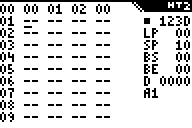
\includegraphics{tut1}} \newline

\begin{tabularx}{\textwidth}{m{0.075\textwidth} X}
\textcolor{red}{\newline\Huge\danger} & Always fill all four positions of a sequence row to avoid glitches and unwanted effects. \\
\end{tabularx} ~\\

\paragraph{Step 3} Move the cursor up to the first position in the sequence again. Now press \textbf{[2nd]}. This will bring up the pattern screen. \newline

{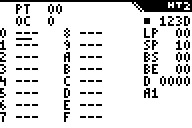
\includegraphics{tut2}} \newline

\paragraph{Step 4} Let's activate RowPlay mode, so we can hear what we're doing. Press \textbf{[ALPHA], [MODE]}.
\paragraph{Step 5} Ok, let's put some notes into this pattern thing. Press \textbf{[PRGM], [PRGM]}.
\paragraph{Step 6} Wow, that's a pretty low note. Let's change the octave by pressing \textbf{[GRAPH], [2]}. Now we can enter some more notes, for example by pressing \textbf{[PRGM], [PRMG], [SIN], [SIN], [TAN], [TAN]}. \newline

{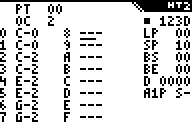
\includegraphics{tut3}} \newline

\paragraph{Step 7} Press \textbf{[ENTER]} to hear what we've got so far.
\paragraph{Step 8} Hmmm, sounds pretty boring, right? So let's spice things up with some drums. Press \textbf{[2nd]} to go back to the main screen. Now move the cursor all the way to the right, and press \textbf{[2nd]} again. This will bring up the Drum/FX pattern screen. \newline

{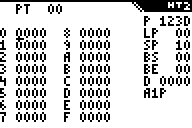
\includegraphics{tut4}} \newline

\paragraph{Step 9} Press \textbf{[1], [\(\medblacktriangledown\)], [2], [2], [1], [\(\medblacktriangledown\)], [2], [2], [1], [\(\medblacktriangledown\)], [2], [2], [\(\medblacktriangledown\)], [2], [\(\medblacktriangledown\)], [2]}. \newline

{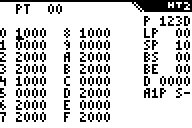
\includegraphics{tut5}} \newline

\paragraph{Step 10} Congratulations, you've just composed your first "song" in HoustonTracker 2!


\section{Keys}
\label{sec:keys}

\begin{center}
{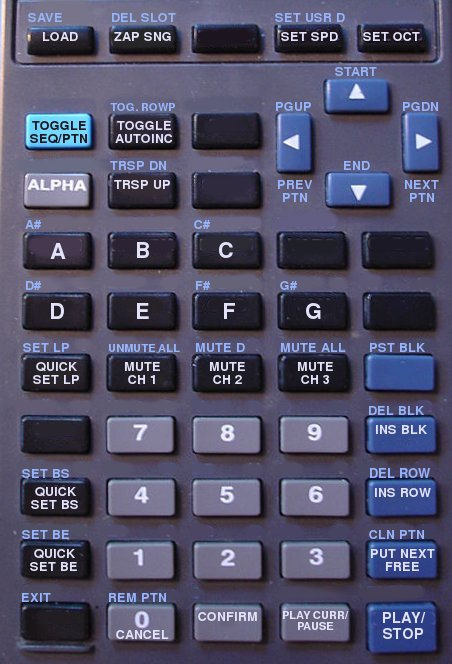
\includegraphics[width=0.75\textwidth]{keymap.jpg}} \newline
\end{center}

\newpage
\begin{longtable}{p{0.35\textwidth} p{0.6\textwidth} }
\textbf{key} & \textbf{function} \\
\hline
%\rowfont\bfseries key & function & description \\ \hline 
%\endhead

\textbf{[ALPHA][ON]} & \textbf{QUIT} HT2. The current tune will be preserved in memory. You can only exit when music isn't playing. On TI83/8x Plus, exiting will take a few moments. \\
\textbf{[Y$\bm{=}$]} & \textbf{LOAD} a song. Prompts prompt for a save slot number (0..7). Needs to be CONFirmed. \\
\textbf{[ALPHA][Y$\bm{=}$]} & \textbf{SAVE} a song. Prompts for a save slot number (0..7). Needs to be CONFirmed. \\
\textbf{[WINDOW]} & \textbf{ZAP}s (clears) the current \textbf{TUNE}. Needs to be CONFirmed. \\
\textbf{[ALPHA][WINDOW]} & \textbf{DEL}ete save \textbf{SLOT}. Prompts for a save slot number (0..7). Needs to be CONFirmed. \\
\hline
\textbf{[.]} & \textbf{CONFIRM} action. (Cancel action with key \textbf{[0]}.) \\
\hline
\textbf{[2nd]} & \textbf{TOGGLE} between \textbf{SEQuence} and \textbf{PaTterN} view. When used on sequence view, it will display the pattern selected by the cursor. \\
\textbf{[ALPHA]} & Toggle \textbf{ALPHA} mode on and off. \\
\hline
\textbf{[MODE]} & Toggle \textbf{AUTOmatic} cursor \textbf{INCrement} on/off (off by default). \\
\textbf{[ALPHA][MODE]} & \textbf{TOGGLE ROWPlay} on and off (off by default). When enabled, plays notes while editing. Beware that \mbox{RowPlay} may ignore some effect settings. \\
\hline
\textbf{[\(\medblacktriangleup\)]} & Move cursor \textbf{UP}. \\
\textbf{[\(\medblacktriangledown\)]} & Move cursor \textbf{DOWN}. \\
\textbf{[\(\medblacktriangleleft\)]} & Move cursor \textbf{LEFT}. \\
\textbf{[\(\medblacktriangleright\)]} & Move cursor \textbf{RIGHT}. \\
\textbf{[ALPHA][\(\medblacktriangleup\)]} & Jump to the \textbf{START} of the sequence. \\
\textbf{[ALPHA][\(\medblacktriangledown\)]} & Jump to the \textbf{END} of the sequence. \\
\textbf{[ALPHA][\(\medblacktriangleleft\)]} & Move one \textbf{PAGE} (10 lines) \textbf{UP} in sequence or select the \textbf{PREVious PaTterN}. \\
\textbf{[ALPHA][\(\medblacktriangleright\)]} & Move one \textbf{PAGE} (10 lines) \textbf{DOWN} in sequence or select the \textbf{NEXT PaTterN}. \\
\hline
\textbf{[ENTER]} & Start \textbf{PLAY}ing from the start of the song, or \textbf{STOP} playback if player is running. \\
\textbf{[$\bm{-}$]} & Start \textbf{PLAY}ing from the \textbf{CURRent} position in sequence, or hold down to \textbf{PAUSE} playback while player is running. \\
\textbf{[ALPHA][$\bm{-}$]} & Start playing and \textbf{LOOP} the \textbf{CURRent} position in sequence. \\
\textbf{[CLEAR]} & Toggle \textbf{HOLD}ing the current row (toggle synth mode) \\
\hline
\textbf{[,]} & \textbf{MUTE}/unmute \textbf{CHannel1}. \\
\textbf{[ALPHA][,]} & \textbf{UNMUTE ALL} channels. \\
\textbf{[(]} & \textbf{MUTE}/unmute \textbf{CHannel2}. \\
\textbf{[ALPHA][(]} & \textbf{MUTE}/unmute \textbf{DRUMS}. \\
\textbf{[)]} & \textbf{MUTE}/unmute \textbf{CHannel3}. \\
\textbf{[ALPHA][)]} & \textbf{MUTE ALL} channels. \\
\hline
\textbf{[0]} & Input \textbf{0} at cursor, \textbf{DELete} a \textbf{NOTE}, or \textbf{CANCEL} action, depending on context. \\
\textbf{[ALPHA][0]} & \textbf{REMove} the currently selected \textbf{PaTterN} from the sequence. \\
\textbf{[1]..[9]} & Input \textbf{1..9} at cursor. \\
\textbf{[MATH]} & Input hex digit or note \textbf{A} at cursor, depending on context. \\
\textbf{[ALPHA][MATH]} & In note pattern view, input note \textbf{A\#} at cursor. \\
\textbf{[MATRIX]/[APPS]} & Input hex digit or note \textbf{B} at cursor. \\
\textbf{[PRGM]} & Input hex digit or note \textbf{C} at cursor. \\
\textbf{[ALPHA][PRGM]} & In note pattern view, input note \textbf{C\#} at cursor. \\
\textbf{[$\bm{x^{-1}}$]} & Input hex digit or note \textbf{D} at cursor. \\
\textbf{[ALPHA][$\bm{x^{-1}}$]} & In note pattern view, input note \textbf{D\#} at cursor. \\
\textbf{[SIN]} & Input hex digit or note \textbf{E} at cursor. \\
\textbf{[COS]} & Input hex digit or note \textbf{F} at cursor. \\
\textbf{[ALPHA][COS]} & In note pattern view, input note \textbf{F\#} at cursor. \\
\textbf{[TAN]} & Input hex digit or note \textbf{G} at cursor. \\
\textbf{[ALPHA][TAN]} & In note pattern view, input note \textbf{G\#} at cursor. \\
\hline
\textbf{[TRACE]} & \textbf{SET} the global song \textbf{SPeeD}. Refer to the section on \nameref{sec:globalvars} for details on this setting. \\
\textbf{[ALPHA][TRACE]} & \textbf{SET} the \textbf{USeR Drum} pointer. Any value between 0x0000 and 0xFFFF is permitted. However, it is recommended to stick with values in the range of 0x0000 - 0x7FFF, as higher values may produce unpredictable results. \\
\textbf{[GRAPH]} & \textbf{SET} the current \textbf{OCTave}. Only works on note pattern screens. Valid values are 0..6. \\
\hline
\textbf{[X,T,$\bm{\Theta}$]} & \textbf{TRanSP}ose current pattern \textbf{UP} by one half-tone. Out-of-range notes will be replaced with rests. \\
\textbf{[ALPHA][X,T,$\bm{\Theta}$]} & \textbf{TRanSP}ose current pattern \textbf{DOWN} by one half-tone. Out-of-range notes will be replaced with rests. \\
\hline
\textbf{[$\bm{x^2}$]} & \textbf{QUICK SET} the \textbf{Loop Point} to the current row in sequence (sequence screen only). Changes will not take effect until the next player restart. \\
\textbf{[ALPHA][$\bm{x^2}$]} & \textbf{SET} a new \textbf{Loop Point} value. Only works on sequence screen. Changes will not take effect until the next player restart. \\
\hline
\textbf{[LN]} & \textbf{QUICK SET} the copy \textbf{Block Start} to the current row in sequence (sequence screen only). \\
\textbf{[ALPHA][LN]} & \textbf{SET} a new copy \textbf{Block Start} value (sequence screen only). \\
\textbf{[STO\(\medblacktriangleright\)]} & \textbf{QUICK SET} the copy \textbf{Block End} to the current row in sequence (sequence screen only). \\
\textbf{[ALPHA][STO\(\medblacktriangleright\)]} & \textbf{SET} a new copy \textbf{Block End} value (sequence screen only). \\
\hline
\textbf{[ALPHA][\(\bm{\div}\)]} & \textbf{PaSTe} the selected \textbf{BLocK} over the current and following rows. The target row must be outside of the selected block. \\
\textbf{[\(\bm{\times}\)]} & \textbf{INSert} the selected \textbf{BLocK} at the current row. \\
\textbf{[ALPHA][\(\bm{\times}\)]} & \textbf{DELete} the selected \textbf{BLocK}. \\
\textbf{[\(\bm{-}\)]} & \textbf{INSert} a copy of the current \textbf{ROW}. \\
\textbf{[ALPHA][\(\bm{-}\)]} & \textbf{DELete} the current \textbf{ROW}. \\
\textbf{[\(\bm{+}\)]} & \textbf{PUT} the \textbf{NEXT} unused \textbf{FREE} pattern in sequence at the current position. \\
\textbf{[ALPHA][\(\bm{+}\)]} & \textbf{CLoNe} the current \textbf{PaTterN} and insert the clone at the current cursor position. \\
\hline
\end{longtable}


\section{Composing Music}
\subsection{Modes, Indicators, and Global Variables}

{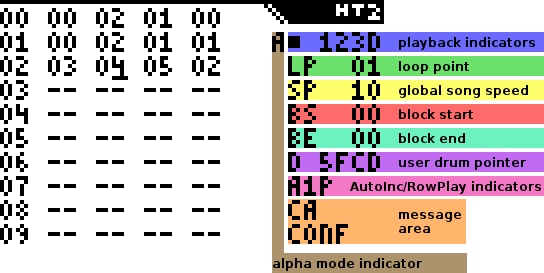
\includegraphics[width=0.75\textwidth]{vars}} \newline

\paragraph{Modes and Indicators} There are a number of different indicators, which will tell you about various modes and editing settings that are currently applied.

The Alpha mode indicator comes in the shape of a capital letter A, which is displayed below the diagonal left edge of the HT2 logo. When the A is visible, then Alpha mode is active. The Alpha mode is HT2's version of the SHIFT key on a PC - except that you press it \emph{before} pressing another key, not together with the second key.
Many keys in HT2 have a primary and secondary function. In Alpha mode, the secondary functions will be triggered. You can toggle Alpha mode on and off by pressing - you guessed it - \textbf{[ALPHA]}. Alpha mode will be turned off automatically once an Alpha mode action has been performed.

The playback indicators are located directly below the HT2 logo. The first position tells you if the music player is currently stopped or running. While stopped, it will display a \(\medblacksquare\), when running, it will display the capital letter P. Next to this position, you will find four positions which normally read "123D" (for channel 1, 2, 3, and drums respectively). These positions indicate which channels are currently muted. Muted channels will display a "-" instead of their channel number/letter.

The AutoInc/RowPlay indicators tell you whether the auto-incrementing and RowPlay functions are currently activated. They are located in the lower third of the right screen side, just below the the global variables. The AutoInc indicator displays "A0" when auto-incrementing is deactivated (default), and A1 when activated. Auto-incrementing means that after you enter a value or note in HT2, the cursor will automatically advance to the next position. You can toggle AutoInc with key \textbf{[MODE]}. The RowPlay indicator tells you whether RowPlay mode is currently active. If so, it will display the capital letter P. When entering a note, HT2 will automatically play the current pattern position (including all channels that are not muted). You can toggle RowPlay by pressing \textbf{[ALPHA], [MODE]}. \newline

\begin{tabularx}{\textwidth}{m{0.075\textwidth} X}
\Huge{\textcolor{red}{\newline\danger}} & RowPlay mode can't reliably detect all effect settings that apply to the current position, so depending on the circumstances, it may not reflect how the position will actually sound when the whole song is played back. \\
\end{tabularx} ~\\

Located to the right of the AutoInc/Rowplay indicators is the saveslot indicator. It will display the last used save slot once the load/save function has been used.

Below the AutoInc/RowPlay indicators, there is the general purpose message area. Here, various important messages will be displayed, such as occuring errors, or requests for the user to confirm an action. Confirming is done with key \textbf{[.]}, cancelling is done with key \textbf{[0]}. 

\paragraph{Global Variables}\label{sec:globalvars} The loop point defines what row in the sequence the player will loop back to after it has reached the end of the song. Pressing \textbf{[$\bm{x^2}$]} will set the loop point to the row currently highlighted by the cursor. To set it to another row, press \textbf{[ALPHA], [$\bm{x^2}$]}, then enter a 2-digit hex number.

The global song speed can be changed by pressing \textbf{[TRACE]}, followed by a 2-digit hex number. The number refers to the number of ticks one row will last. So generally speaking, a higher number means lower speed.

Any number in the range of 0x01 - 0x3F will set the number of ticks directly. Adding 0x40 to the value will reduce the length of the first tick by ¾, adding 0x80 will reduce it by ½, and adding 0xc0 will reduce it by ¼. Thus, setting the speed to 0x08 will result in a row length of 8 ticks, 0xc8 will result in a row length of 7¾ ticks, 0x88 will result in a row length of 7½ ticks, and 0x48 will result in a row length of 7¼ ticks. Note that reducing the length of the first tick will have a noticable impact on various effects including 2xx/3xx (pitch slides), 8xx (execute note table), and Cxx (note cut).

0x00 (aka the "drone mode") is an exception. It is the slowest possible setting, equivalent to a row length of 256 ticks (minus a fraction of a tick when adding using 0x40/0x80/0xc0).

To set the user drum pointer, press \textbf{[ALPHA], [TRACE]}, followed by a 4-digit hex number. See the section on \nameref{sec:drums} for details about the user drum pointer. \newline

\begin{tabularx}{\textwidth}{m{0.075\textwidth} X}
{\textcolor{red}{\newline\Huge\danger}} & Changes to the global variables are not effective until you restart the player. \\
\end{tabularx} ~\\


\subsection{Editing the Song Sequence}

{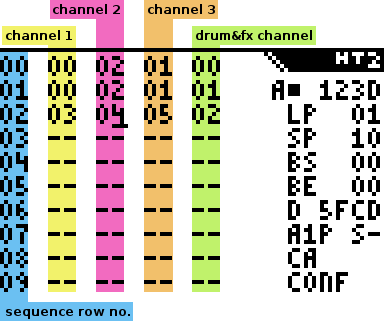
\includegraphics[width=0.6\textwidth]{seq}} \newline

The sequence screen is where you build the general structure of your song. It consists of four editable columns, each containing a list of patterns. Each column represents a different channel. To toggle between the main (sequence) screen and the pattern screens, select a pattern in the sequence with the cursor, then press \textbf{[2nd]}.

The first 3 columns represent the 3 tone channels, ie. they contain \hyperref[sec:notepat]{note patterns}. The last column represents the drum channel and effects settings, ie. it contains \hyperref[sec:fxpat]{fx patterns}. The tone channels differ somewhat in sound and features. Channel 1 features a note cut \nameref{sec:fx}. It can also play noise and  glitchy sounds in addition to the regular tone. Channel 2 is somewhat louder than the other channels, and features some advanced duty modulation effects, including a SID-style duty cycle sweep. Channel 3 features pitch slides, note (arpeggio) tables, and another set of glitch sounds. All channels support a variable duty cycle.

\paragraph{Moving around on the sequence screen} Keys \textbf{[\(\medblacktriangleup\)], [\(\medblacktriangledown\)], [\(\medblacktriangleleft\)]}, and \textbf{[\(\medblacktriangleright\)]} move the cursor around on the sequence screen. Pressing \textbf{[ALPHA], [\(\medblacktriangleleft\)]} resp. \textbf{[ALPHA], [\(\medblacktriangleright\)]} will move the cursor up/down by 10 rows. Pressing \textbf{[ALPHA], [\(\medblacktriangleup\)]} will move the cursor to the start of the sequence. Likewise, pressing \textbf{[ALPHA], [\(\medblacktriangleup\)]} mode will move the cursor to the end of the sequence.

\paragraph{Editing the sequence} Use keys \textbf{[0]..[9]} and A..F (\textbf{[MATH], [MATRX]} resp. \textbf{[APPS], [PRGM], [$\bm{x^{-1}}$], [SIN]}, and \textbf{[COS]}) to enter pattern numbers. You can have a maximum of 128 note patterns, and 64 fx patterns, so the highest pattern numbers are 0x7F and 0x3F respectively. Note patterns are shared across all 3 tone channels, so you can use any note pattern on any channel. If you try to enter an invalid pattern number, HT2 will automatically replace it with an arbitrary valid one.

\begin{tabularx}{\textwidth}{m{0.075\textwidth} X}
{\textcolor{red}{\newline\Huge\danger}} & Note patterns and fx patterns use a different numbering, e.g. note pattern 01 is different from fx pattern 01. \\
\end{tabularx} ~\\

To automatically put the first unused pattern at the current sequence position, press \textbf{[$\bm{+}$]}. To clone the pattern at the current position (copy it's contents to a new, unused pattern), press \textbf{[ALPHA], [$\bm{+}$]}. To delete the pattern number at the current position, press \textbf{[ALPHA], [0]}.

You can press \textbf{[$\bm{-}$]} to copy the current row. This will insert the copy at the current position. Press \textbf{[$\bm{-}$]} to delete the current row.

\begin{tabularx}{\textwidth}{m{0.075\textwidth} X}
\Huge{\textcolor{red}{\newline\danger}} & Always fill all four sequence positions in a given row. Pressing play on a sequence row that has empty positions will have undesired side effects. \\
\end{tabularx} ~\\

\paragraph{Block Operations} HT2 uses two block markers, block start (BS) and block end (BE) to select a section of sequence data for copying, pasting, and cutting. Block operations work only on the whole sequence, not on individual channels.

To set the block start to the current row in the sequence, press \textbf{[LN]}. Likewise, to set the block end to the current row, press \textbf{[STO\(\medblacktriangleright\)]}. Pressing these keys in \textbf{[ALPHA]} mode will allow you to set the BS/BE positions manually.

To copy the marked block and insert it at the current cursor position, press \textbf{[\(\bm{\times}\)]}. Pressing \textbf{[ALPHA], [\(\bm{\div}\)]} will paste the block over the following sequence rows. Note that you cannot insert/paste a block into itself, so the target must always be outside the selected block.

Press \textbf{[ALPHA], [\(\bm{\times}\)]} to delete the selected block and move the following sequence data up.


\subsection{Editing Note Patterns}
\label{sec:notepat}

{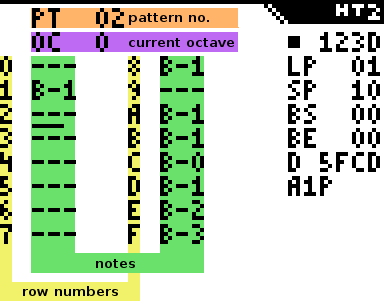
\includegraphics[width=0.6\textwidth]{noteptns}} \newline

All note patterns have a fixed length of 16 steps, which are organized in two columns à 8 steps.

Notes can be entered with keys \textbf{[MATH]} (A), \textbf{[MATRX]} resp. \textbf{[APPS]} (B), \textbf{[PRGM]} (C), \textbf{[$\bm{x^{-1}}$]} (D), \textbf{[SIN]} (E), \textbf{[COS]} (F), and \textbf{[TAN]} (G). Sharp notes (black keys) can be reached with \textbf{[ALPHA]} + note key.

In order to hear notes while you're entering them, you can toggle RowPlay by pressing \textbf{[ALPHA], [MODE]}. A "P" will be displayed next to the AutoInc indicator to let you know that RowPlay is active. Note that RowPlay is somewhat limited. Among other things, it may ignore current effect settings. Also, it will fail if the pattern you're editing is not on the current step in the song sequence.

To change the current octave, press \textbf{[GRAPH]}, then enter a number between 0 and 6. You can also edit octaves manually in the pattern.

\begin{tabularx}{\textwidth}{m{0.075\textwidth} X}
{\textcolor{black}{\newline\Huge\PointingHand}} & You can cycle through note patterns with \textbf{[ALPHA], [\(\medblacktriangleleft\)]} and \textbf{[ALPHA], [\(\medblacktriangleright\)]}. \\
{\textcolor{black}{\newline\Huge\PointingHand}} & In order to use a different pattern length, use the \hyperref[sec:fx]{B00 effect command}. \\
\end{tabularx} ~\\


\subsection{Editing Drum/Effects Patterns}
\label{sec:fxpat}

{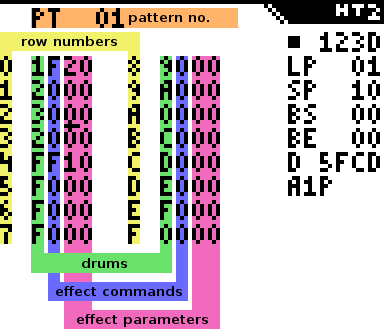
\includegraphics[width=0.6\textwidth]{fxptns}} \newline

Like with note patterns, fx patterns are organized in two columns à 8 steps. Each step consists of four hex digits. The \emph{first digit} sets the drum sound to be used on that step. A value of 0 means no drum. Refer to the \hyperref[sec:drums]{following section} to learn more about drums in HT2.

The \emph{second digit} sets the effect command. A value of 0 means no effect. Finally, the \emph{last two digits} set the effect parameters. Refer to the \nameref{sec:fx} to learn all about effects. 


\subsubsection{Drums}
\label{sec:drums}

There are 15 different drums to chose from (0x1..0xF). Some of the drums use the TI-OS as sample data, so their sound may vary across different calculator models.

Drums can be played in different modes, which affects the way they sound. Use command Cxx to change the drum mode, with xx = 0x00..0x4f. There are 80 different drum modes, though not all of them are particularly useful.

Setting a non-zero value for the \emph{lower nibble} of the parameter causes the drum data to be manipulated in various ways. Refer to the appendix on \nameref{sec:synthtec} for details about this functionality.

The \emph{upper nibble} of the parameter defines the behaviour of the drum data pointer. The effects are as follows: \newline

\begin{tabularx}{\textwidth}{p{0.1\textwidth} p{0.1\textwidth} X}
\textbf{mode} & \textbf{cmd} & \textbf{effect} \\
\hline
0 & C00 & Increment pointer, ie. use the "standard" drum set. \\
1 & C1x & Decrement pointer, ie. use the "alternative" drum set. Generally speaking, these drums are less useful than the standard set. Also, some drums will produce unpredictable results, namely drum 0, 1, C, and D. \\
2 & C2x & Increment and loop pointer. Even less useful than mode 1, and suffers from the same problems. Also, this mode causes a slight global pitch shift. \\
3 & C3x & Decrement and loop pointer. Like mode 2, with different sounds. \\
4 & C4x & Don't move pointer. Instead of drums, in this mode triggering a drum will play a fixed, most likely out-of-tune frequency. This mode causes a slight global pitch shift. \\
\end{tabularx} ~\\

Drum 0xE and 0xF are special cases.

0xF is the user drum pointer, which can be configured individually. To change it, press \textbf{[ALPHA], [TRACE]}.
The user drum pointer can be set to any value between 0x0000 and 0xFFFF. However, if you want to play it safe you should keep the pointer in range 0x0000 - 0x7FFF. This is because the user drum is actually a pointer to ROM/RAM. Pointing the user drum to RAM (0x8000 and up) will give unpredictable results, as the RAM contents change frequently.

0xE is the user defined sample. This feature is a bit quirky in use. In order to create a custom sample, go to FX pattern 0x20. Now, instead of entering the usual drum triggers, fx commands, and fx parameters, you enter your sample data. You can use more than one pattern, so after you've filled up FX pattern 0x20, go to 0x21.

The data is in 1-bit PWM format, meaning each byte denotes a phase length. Think of it as the amount of time taken until the beeper output will toggle again. The values are inverse, ie. a lower value denotes a longer phase. Yes, it's a bit confusing... As an example, this is what drum sample 1 (the kick drum) looks like:
\begin{verbatim}
0x80, 0x80, 0x70, 0x70, 0x60, 0x60, 0x50, 0x50, 0x40, 0x40, 
0x40, 0x30, 0x30, 0x30, 0x30, 0x20, 0x20, 0x20, 0x20, 0x20, 
0x10, 0x10, 0x10, 0x10, 0x10, 0x10, 0x8, 0x8, 0x8, 0x8, 0x8, 
0x8, 0x8, 0x4, 0x4, 0x4, 0x4, 0x4, 0x4, 0x4, 0x4, 0x2, 0x2, 
0x2, 0x2, 0x2, 0x2, 0x2, 0x2, 0x2, 0x0
\end{verbatim}

This will give you a waveform looking like this: \newline

{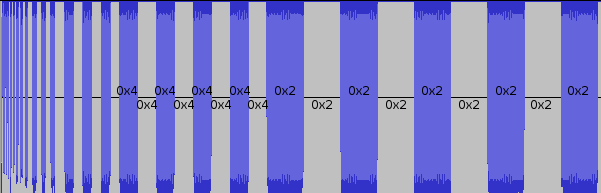
\includegraphics[width=\textwidth]{drumwave}} \newline

\begin{tabularx}{\textwidth}{m{0.075\textwidth} X}
{\textcolor{red}{\newline\Huge\danger}} & The last byte of the sample must be 0. \\
\Huge{\textcolor{black}{\newline\PointingHand}} & You can even define a second drum sample, which you can then trigger in drum mode C1x/C3x. This sample also starts at FX pattern 0x20, but needs to be written backwards, so the second byte of the sample is on the last position (FX parameter of the last row) of FX pattern 0x1F, third byte is just before that (drum/FX command of the last row), and so forth. \\
\end{tabularx} ~\\

\newpage
\subsubsection{Effects Reference}
\label{sec:fx}

\begin{longtable}{p{0.1\textwidth} p{0.2\textwidth} p{0.6\textwidth}}
\textbf{cmd} & \textbf{effect} & \textbf{description} \\
\hline
1xx & SET PAN & Set panning for all channels. To determine how the panning will be set, you need to look at the individual bits of the effect parameter, starting at the rightmost one (aka bit 0). \newline

bit 0 set: pan ch1 right (add 0x1 to xx)

bit 1 set: pan ch1 left (add 0x2)

bit 0,1 reset: pan ch1 center (add nothing)

bit 2 set: pan ch2 right (add 0x4)

bit 3 set: pan ch2 left (add 0x8)

bit 2,3 reset: pan ch2 center (add nothing)

bit 4 set: pan ch3 right (add 0x10)

bit 5 set: pan ch3 left (add 0x20)

bit 4,5 reset: pan ch3 center (add nothing)

bit 6 set: pan drums right (add 0x40)

bit 7 set: pan drums left (add 0x80)

bit 6,7 reset: pan drums center (add nothing) \newline

\textbf{Examples:} \newline

\emph{Pan all channels to center}

0x0 + 0x0 + 0x0 + 0x0 = 0x0 $\rightarrow$ use 100 \newline

\emph{pan all channels right}

0x1 + 0x4 + 0x10 + 0x40 = 0x55 $\rightarrow$ use 155 \newline

\emph{pan ch1 left, ch2 center, ch3 right, drums center}

0x2 + 0x0 + 0x10 + 0x0 = 0x12 $\rightarrow$ use 112 \newline

If you're having trouble figuring out the right values, you can use this \href{http://garvalf.online.fr/temp/ht2_panning.html}{online tool by garvalf} to calculate the parameters. \\
\hline
2xx & PITCH SLIDE UP CH3 & Perform an upward pitch slide on channel 3.

xx defines the speed of the slide, lower values mean slower slides. xx can be any value, but beware that the pitch counter will eventually wrap.

200 disables the effect. \\
\hline
3xx & PITCH SLIDE DOWN CH3 & Perform a downward pitch slide on channel 3. Using this will disable effect 9xx.

xx defines the speed of the slide, lower values mean slower slides. xx can be any value, but beware that the pitch counter will eventually wrap.

300 disables the effect. \\
\hline
4xx & DUTY CYCLE/NOISE CH1 & Set the duty cycle for channel 1, and toggle noise mode.

xx \textless= 0x80 - set duty cycle and disable noise mode

xx \textgreater\space0x80 - set duty cycle and enable noise mode \\
\hline
5xx & DUTY CYCLE/SWEEP CH2 & Set the duty cycle for channel 2, or enable duty cycle sweep.

xx \textless= 0x80 - set duty cycle and disable duty cycle sweep. A value of 0x80 produces the default 50:50 wave. Very low values will cause glitches.

xx \textgreater\space0x80 - enable SID-style duty cycle sweep. Sweep speed = (xx \& 0x7F), 581 will produce the classic sweep effect known from HT versions \textless= 2.20.

Some parameters are shared with effect 7xx, hence these two effects impact each other. \\
\hline
6xx & DUTY CYCLE/GRIND CH3 & Set the duty cycle for channel 3, and toggle grind mode.

xx \textless= 0x80 - set duty cycle and disable grind mode.

xx \textgreater\space0x80 - set duty cycle to (xx*2)\&0xff and enable grind mode. \\
\hline
7xx & AUTO CHORD CH2 & Add a chord effect to channel 2.

xx \textless\space0x80 - enable unsynced auto chord. The chord created varies depending on the note used, and is not necessarily harmonic.

xx \textgreater= 0x80 - enable synced auto chord. This will produce an octave chord, depending to some extend on the current duty setting. A higher value for xx will generally produce stronger harmonics.

700 switches off the effect.

Some parameters are shared with effect 5xx, hence these two effects impact each other. See the description of effect 5xx for details. \\
\hline
8xx & EXEC NOTE TABLE CH3 & Execute a given pattern as a note table for channel 3. This effect operates on a per-tick basis. Execution starts after the first tick.

xx is the pattern to be executed as note table. If the current tempo is greater than 0x10, table execution will continue at the following pattern.

To disable the effect, set xx to a value greater than 0x7F.

Using this effect will disable the Cxx (note cut ch1) effect. \\
\hline
9xx & GLITCH CH3 & Add a nasty glitch effect to channel 3.

xx can be any value, 900 turns off the effect. \\
\hline
Axx & CH3 PHASE & Set the phase offset for channel 3.

This has little effect on itself, but will cause interference when used together with another channel that plays the same note as ch3. In this case, it can be used as a primitive form of volume control.

xx can be any value, values around 0x80 will work best. A00 turns off the effect. \\
\hline
Bxy & BREAK PTN/LOOP SECTION & xy = 0 - break pattern immediately and jump to the next position in the sequence. B00 is ignored on the first line of a pattern.

xy \textgreater\space0 - jump back y rows in the pattern, repeating the section x times.

The Bxy effect should not be nested (ie. don't put a Bxy loop within another Bxy loop), because doing so will lead to an infinite loop. Beware, HT2 does not check this. \\
\hline
Cxx & NOTE CUT CH1 & Cut the note on channel 1 after xx ticks. Using this effect can make the sound output slightly more noisy.

Use C00 to disable the effect.

Using this effect will disable the 8xx (exec note table ch3) effect. \\
\hline
Dxx & DRUM MODE & Set the drum mode, where xx is 0x00..0x4F. Refer to the \nameref{sec:drums} section for details. \\
\hline
Exx & EXTENDED FX & Various extended effects. Using this effect causes a slightly longer than normal delay when triggered, leading to additional transition noise.

Exx with xx \textless\space0x40 - execute up to 5 effects stored at the start of effects pattern xx at once. Effects Bxx and Exx will be ignored.

E80 - reset all effects and restore global variables to their defaults.

E81 - as above, but does not reset speed.

E82 - as above, but does not reset speed and duty cycles.

E83 - as above, but does not reset speed, duty cycles, and panning settings. \\
\hline
Fxx & SET SPEED & Set the current speed. This command temporarily overrides the global speed setting, but does not permanently change it. For details on how the speed setting works, refer to the section on \hyperref[sec:globalvars]{global variables}.

TIP: When entering this effect while the player is running, make sure to enter the parameter first, and then the F command. \\
\hline
\end{longtable} ~\\


\section{Loading, Saving, and Backing Up}
\paragraph{Saving} To save your current work in progress, press \textbf{[ALPHA], [Y$\bm{=}$]}. The letters "SA" will appear in the message area. Now, enter the number of the save slot you want to save (0..7), and confirm by pressing \textbf{[.]}. (If you got here by accident, press \textbf{[0]} to cancel.)

If the save was successful, error code E0 will be displayed in the message area. If the save was unsuccessful due to insufficient memory, error code E2 will be displayed instead. Note that you may run out of memory rather quickly. You will always be able to maintain at least two save slots, however. \newline

\begin{tabularx}{\textwidth}{m{0.075\textwidth} X}
{\textcolor{red}{\newline\Huge\danger}} & Any data after the first unfilled position (- -) in the sequence is \emph{not} saved. \\
\end{tabularx} ~\\

\paragraph{Loading} To load a previously saved tune, simply press \textbf{[Y$\bm{=}$]}. The letters "LD" will appear in the message area.
Now, enter the number of the save slot you want to load (0..7), and confirm by pressing \textbf{[.]}. (If you got here by accident, press \textbf{[0]} to cancel.)
The tune in question will be loaded, or error code E5 will be printed if the selected save slot was empty.

\paragraph{Deleting a save slot} In case you run out of memory, or want to get rid of one of your save slots for other reasons, you can specify a save slot to be deleted. In order to do so, press \textbf{[ALPHA], [WINDOW]}. The letters "DS" will appear in the message area. Now, enter the number of the save slot you want to delete (0..7), and confirm by pressing \textbf{[.]}. (If you got here by accident, press \textbf{[0]} to cancel.)
And that's all you need to know about deleting save slots!

\paragraph{Backups} Creating a backup of your HT2 songs is trivial: Simply send the HT2 PRGM file to your computer or another calc of the same model. The program file contains all the save slots as well as the currently loaded song. \newline

\begin{tabularx}{\textwidth}{m{0.075\textwidth} X}
{\textcolor{black}{\newline\Huge\PointingHand}} & You can use the \hyperref[sec:ht2util]{ht2util savestate manager} to extract/insert save slots into your HT2 PRGM file. \\
\end{tabularx} ~\\


\section{Error Codes}
If a major error happens, HT2 will attempt to detect it, and print an error code in the message area. An special error message will also be displayed if saving a backup of the current song was successful.

The following table lists all possible error codes: \newline

\begin{tabularx}{\textwidth}{p{0.1\textwidth} X}
\textbf{code} & \textbf{description} \\
\hline
E0 & \textbf{SAVE OK:} Saving backup was successful, no error occured. \\
E1 & \textbf{INVALID BLOCK:} Block End is set before Block Start, or the row where the block should be inserted/pasted to is within the selected block. \\
E2 & \textbf{INSUFFICIENT MEMORY:} There is not enough RAM to perform the desired action (usually saving). \\
E3 & \textbf{INVALID PTN:} An invalid pattern number was set in the song sequence. \\
E4 & \textbf{LP INVALID:} Invalid loop point. Row to loop to is empty. \\
E5 & \textbf{FILE I/O ERR:} Loading song failed. Save slot is empty or corrupt. \\
E6 & \textbf{SAVESTATE ERR:} Wrong savestate version, or savestate corrupt. \\
E7 & \textbf{NO FREE PTN:} Could not find a free pattern. \\
E8 & \textbf{BLOCK TOO LARGE:} The selected block is too large to be inserted. \\
\end{tabularx} ~\\


Small errors (like trying to set an inexistent note or an invalid pattern number) will be simply ignored by HT2.

\chapter{The ht2util Savestate Tool}
\label{sec:ht2util}
\paragraph{ht2util} is a PC-based savestate manager application for HoustonTracker 2. It allows you to export and import songs from/to the savestate block of your HT2 binary, among other things.

Even though ht2util comes bundled with HT2 releases, it is maintained seperately. Check the \href{https://github.com/utz82/ht2util/releases}{ht2util git} for the latest version.

\paragraph{Installation} ht2util works as a stand-alone application, no installation is required. Linux users can compile the program from source by running "make" in the /ht2util-gui directory. ht2util depends on wxWidgets 2.8 or higher, so install that first if necessary. Most Linux distros provide a native wxWidgets implementation in their repositories.

\paragraph{Usage} Always start by loading a HT2 program file. This can be a blank ht2.8*p, or one you've backed up from your calculator. Once the file has loaded successfully, the contents of its savestate table will be displayed in the left panel.

To \emph{import} a savestate, use "File$\rightarrow$Insert savestate...", or drag one or more files from the right-hand (filebrowser) panel to the left-hand (savestate) panel. If the savestate was extracted from an older version of HT2, ht2util will offer to automatically upgrade the it. This will always work with stable HT2 releases (except for some effects/settings that can not be upgraded automatically), but might, in rare cases, cause some problems with beta versions.

To \emph{delete} one or more savestates, mark the desired state(s) in the savestate panel, then use "File$\rightarrow$Delete savestate" or simply press "Delete".

To \emph{extract} one or more savestates, mark the desired state(s) in the savestate panel and then use "File$\rightarrow$Extract savestate..." to save it with a ".ht2s" extension. You can also simply drag the desired savestate(s) from the savestate panel to the filebrowser panel; this will save the state(s) with a generic filename.

Furthermore, you can decompress and export savestates to .asm, however this is not particularly useful yet unless you're working with the HT2 source. \newline

\begin{tabularx}{\textwidth}{m{0.075\textwidth} X}
\Huge{\textcolor{red}{\newline\danger}} & ht2util does not automatically update effect commands yet. If you've imported a savestate from an older version of HT2, you will need to adjust those manually. Refer to the changelog to see which commands need to be updated. \\
\end{tabularx} ~\\


\chapter{Thanks, Credits, and Greetings}


Thanks to... \newline

\begin{easylist}[itemize]
& TylerBarnes, Tronimal, garvalf, Flashbob, giako9000, nonfinite, and Imaginary for beta testing
& Jankenpopp and unexpectedbowtie for figuring out the install process under non-standard configurations
& extra thanks to garvalf for preparing the HT2 cheatsheet
& Shiru, introspec, and Alone Coder for their expertise and advice
& Brandon Wilson, Lionel Debroux, Benjamin Moody, critor, and everybody who has been hacking/documenting TI calcs \newline
\end{easylist}

The TI-82 image that was used as the basis of the keymap was authored by Martin Olsson, and is released under a \href{https://gnu.org/licenses/fdl.html}{GFDL}/\href{https://creativecommons.org/licenses/by-sa/3.0/}{Creative Commons BY-SA} license.


\begin{appendices}
\chapter{Building from Source}

The latest version of the HT2 source code can always be found at \href{github.com/utz82/HoustonTracker2}.

HoustonTracker 2 is developed under Linux. If you're running Linux or another *nix derivate, building HT2 is a matter of simply running the build script, provided you have a few basic tools installed. If you're developing on Windows or another non-Posix compliant system, you'll need to provide your own build script or build from hand.

\paragraph{Building Requirements} ~\\
\begin{easylist}[itemize]
& The \href{http://pasmo.speccy.org/}{Pasmo assembler} must be installed and present in your search path (unless you want to adapt the sources for another assembler).
& Optionally, you may want to install an TI calculator emulator. For *nix systems, using the development version of tilem2 is recommended.
\end{easylist}

\paragraph{Building with the Build Script (*nix only)} It's as simple as opening a terminal, navigating to the folder containing HT2, and typing

\begin{alltt}
./compile.sh \emph{-[model]}
\end{alltt}

where \emph{[model]} is one of

\begin{tabularx}{\textwidth}{p{0.1\textwidth} X}
82 & build for TI-82 \\
8p & build for TI-82 Parcus \\
83 & build for TI-83, TI-82 Stats \\
8x & build for TI-83 Plus, TI-84 Plus etc. \\
8xs & build "small" version for TI-83 Plus, TI-84 Plus etc. \\
all & build all targets. \\
\end{tabularx} ~\\

Optionally, you can rebuild the note table before running the build script. In order to do so, run the tablegen.sh shell script. This will allow you to change HT2's base tuning.

In order to have the build script automatically run your builds in tilem2, uncomment the lines in compile.sh that look like this:

\begin{alltt}
tilem2 -a -r "\emph{/path/to/your/rom/xyz.rom}" -m \emph{[model] [buildfile]}
\end{alltt} ~\\

\paragraph{Building by Hand} The following steps are required to build HT2 by hand: 

1. Assemble the sources with the following command:

\begin{alltt}
pasmo --equ MODEL=\emph{[model]} --alocal main.asm main.bin
\end{alltt}

where \emph{[model]} can be either 1 (TI-82 build), 2 (TI-83 build), 3 (Plus models build), 4 (TI-82 Parcus build), or 5 (Plus models small build).

2. Pack the resulting main.bin into a TI executable (82p, 83p, 8xp) using a packer of your choice (oysterpac, bin8x, etc...).



\chapter{Data Format Specification}

\paragraph{Work Area Data Format} The work area is where HT2 stores the currently loaded song. It begins at label "musicData", and is 5125 bytes in size. The actual address in memory depends on the version of HT2. \newline

\begin{tabularx}{\textwidth}{p{0.1\textwidth} p{0.1\textwidth} X}
\textbf{offset} & \textbf{length} & \textbf{description} \\
\hline
+0 & byte & global speed \\
+1 & word & user drum pointer \\
+3 & byte & loop point \\
+4 & 1 KB & pattern sequence list. 1 byte per pattern. Order is ch1, ch2, ch3, fx. Empty positions are filled with 0xFF. \\
+1028 & byte & one 0xFF byte to mark the end of the sequence list. \\
+1029 & 2 KB & note patterns. Each note pattern has an uncompressed length of 16 bytes. Empty positions contain 0x00. \\
+3077 & 2 KB & FX patterns. Each fx pattern has an uncompressed length of 32 bytes. Empty positions contain 0x00. \\
\end{tabularx} ~\\

\paragraph{Compressed Savestate Format} HT2 uses a very simple compression scheme to store song data backups. They are set up as follows:

\begin{tabularx}{\textwidth}{p{0.1\textwidth} p{0.1\textwidth} X}
\textbf{offset} & \textbf{length} & \textbf{description} \\
\hline
+0 & byte & global speed \\
+1 & word & user drum pointer \\
+3 & byte & loop point \\
+4 & ? & pattern sequence list. 1 byte per pattern. Order is ch1, ch2, ch3, fx. \\
? & byte & one 0xFF byte to mark the end of the sequence list. \\
? & ? & note patterns.

if byte value at offset \textgreater= 0xE0, then the following (value - 0xDF) patterns are empty.

else, if byte at offset \textgreater= 0xD0, then the following (value - 0xCF) rows are empty.

else, if byte at offset \textless\space0xD0, it's a regular note value. \\
? & byte & one 0xFF byte to mark the end of the note pattern area. \\
? & ? & FX patterns.

FX patterns are preceded by their pattern number. A pattern number of 0xFF signals that the savestate contains no FX patterns.

If bit 7 of the pattern number is set, it's the last pattern to be loaded. Setting bit 7 is optional if the last saved FX pattern is 0x3F. \\
\end{tabularx} ~\\

Start and end addresses of backup savestates are stored in the savestate lookup table, which is located directly before the compressed savestate buffer. Since version 2.20, the savestate LUT is marked in memory with the ASCII string "XSAVE".




\chapter{Synthesis Techniques}
\label{sec:synthtec}
\emph{The information given in this appendix may be out of date, and may not provide an accurate description of the techniques used in the current version of HT2.}

The following section describes how the multi-channel synthesis is achieved in HT2, and how the effects are produced.

\paragraph{General Notes} Sound mixing in HT2 is achieved through a 1-bit synthesis technique called Pulse Interleaving.

Typically, a 1-bit DAC can only output one single square wave frequency. What Pulse Interleaving does is interlace the multiple software channels at a rapid rate. Due to their own hardware latency, common output devices such as speakers or headphones cannot fully adjust their speaker cones at this rate. Therefore the cones will be left in a floating state between full extension and full contraction. This is how the different volume levels needed to mix HT2's four software channels are achieved.

The average time taken to interlace one sample of all 4 channels is (1/16300)s, meaning channel states are swapped at a rate of about 65200 Hz. The exact timings depend on various factors such as actual tone frequencies, effect and drum settings, hardware model, and battery state.


\paragraph{Tone Channels} Once per interlacing cycle, a 16-bit constant (the "frequency base value") is added to a 16-bit counter. The hi-byte of the counter is then compared against a threshold value. If the threshold constant is greater than the hi-byte of the add counter, the output state will be high (1), otherwise it will be low (0).

The threshold value determines the duty cycle ratio. When the threshold is 0x80, the output state will be high 50\% of the time, and low for the other 50\%. When the threshold is, say, 0x40, the ratio will be 25\%:75\%.

The 9xx effect (glitch channel 3) is achieved by constantly rotating the hi-byte of the base frequency value. Similarly, the A01 effect (noise/glitch channel 1) is achieved by rotating the hi-byte of the add counter. This may or may not generate enough pseudo-randomness to produce a noise-like effect, depending on the frequency base value.

The D01 effect (duty cycle sweep) is achieved by incrementing the threshold value once every interlacing cycle. As it is an 8-bit value, it will wrap to 0 once it reaches 0xFF.

The pitch slides are achieved by adding a constant to the frequency base value once per interlacing cycle.

\paragraph{Drum Channel} Drums are generated from values in either ROM or RAM. The values read will be interpreted as 8-bit counters, which are decremented once per interlacing cycle. When the counter reaches 0, the output state of the drum channel is toggled, and the next value is read from ROM/RAM. When a 0-byte is read, the output stops.

Drums 0x1, 0xC, and 0xD are hard-coded in RAM. The "user drum sample" (drum 0xE) is effectively a pointer to FX pattern 0x20. The "user drum pointer" (drum 0xF) is a simple user-definable pointer which can point to either RAM or ROM. All other drums point to ROM, which explains why they sound different depending on what calculator model is used.

The "drum mode" effect (Cxx) will do two things. The upper nibble of the effect parameter determines the direction of the ROM/RAM pointer used to retrieve the counter values. If the upper nibble is 0, the pointer will move forward. If 1, it will move backward. If 2 or 3, only the lo-byte of the pointer will be in/decremented, which means the pointer stays on the same 256-byte memory page. If 4, the pointer will not be moved at all.

The lower nibble of the effect parameter will determine how the values are modified after they are read from memory. The manipulations are as follows: \newline

\begin{tabularx}{\textwidth}{p{0.1\textwidth} X}
\textbf{value} & \textbf{effect} \\
\hline
0x0 & no manipulation \\
0x1 & transform into binary coded decimal \\
0x2 & multiply by 2 \\
0x3 & divide by 2 \\
0x4 & 1's complement \\
0x5 & use lo-byte of pointer as value \\
0x6 & add lo-byte of pointer \\
0x7 & add hi-byte of pointer \\
0x8 & subtract hi-byte of pointer \\
0x9 & subtract lo-byte of pointer \\
0xA & logical AND with hi-byte of pointer \\
0xB & logical AND with lo-byte of pointer \\
0xC & logical OR with hi-byte of pointer \\
0xD & logical OR with lo-byte of pointer \\
0xE & exclusive OR with hi-byte of pointer \\
0xF & exclusive OR with lo-byte of pointer \\
\end{tabularx} ~\\


In some drum modes, the drum channel will produce sound even if a 0-byte is encountered in the data. This is due to the fact that the modifications are applied before checking if the value read from memory is 0.

For a more detailed description on 1-bit sound techniques, check out \href{http://randomflux.info/1bit/viewtopic.php?id=21}{How to Write a 1-Bit Music Routine} on the 1-bit Forum.

\chapter{Troubleshooting}
\label{sec:troubleshoot}
\section{I'm having problems installing/configuring TiLP on Windows.}
\paragraph{I'm getting weird errors when trying to install/run TiLP on Vista/ 7/8/10.} Check the \href{https://github.com/debrouxl/tilp_and_gfm/blob/master/tilp/trunk/README.win32}{extended Win32 readme}, it has solutions for the most common problems.

\paragraph{TiLP refuses to run on my Windows XP.} Windows XP is no longer supported in TiLP2 1.17. You'll need to use an older version.

\paragraph{TiLP fails to fetch the GTK+ installer.} You need to install the \href{http://sourceforge.net/projects/gladewin32/files/gtk+-win32-devel/2.12.9/}{GTK+  package} manually. Afterwards, make sure you uncheck the GTK+ installation box in the TiLP installer.

\paragraph{My TI-82 isn't auto-detected.} That's ok, just configure the Device Settings manually and you should be good to go.

\section{I can't figure out how to install TiLP on OS X.}
An easy way to install TiLP is by using \href{https://guide.macports.org/}{MacPorts}. After you have set up MacPorts, you can install TiLP with the command

\begin{verbatim}
[sudo] port install tilp2
\end{verbatim}

Thanks to unexpectedbowtie for coming up with this solution!

Alternatively, you could use the official \href{https://education.ti.com/en/us/products/computer_software/connectivity-software/ti-connect-software/tabs/overview}{TI-Connect} linking software. However, TI-Connect does not fully support the TI82, so you won't be able to upload HT2 on that model. Alternatively, you could run Linux in a virtual machine, and use TiLP from there.

\section{How do I configure my GrayLink cable under Windows?}
\paragraph{1. Install a driver for GrayLink} ~\\
\begin{easylist}[enumerate]
& boot computer and do not plug your link device
& If your graylink cable is PL2303TA based, you need this \href{http://www.prolific.com.tw/US/ShowProduct.aspx?p_id=153&pcid=41}{specific usb-serial driver} (others will not work)
& plug your link device then check in your device Manager to see if everything is ok, set the COM port to 1, 2, 3 or 4... more than 4 will not work.
& unplug your link device
& reboot computer
\end{easylist}

\paragraph{2. Install TILP2} ~\\
\begin{easylist}[enumerate]
& do not plug the link device
& first install \href{http://sourceforge.net/projects/gladewin32/files/gtk+-win32-devel/2.12.9/}{GTK+ 2.12.9-win32} dependencies
& then install \href{http://lpg.ticalc.org/prj_tilp/win32.html}{TiLP} (be sure to uncheck GTK+ installation box, because you already did it)
& plug the link device
& open TILP, then 'control+D' and set your connection parameters:
&&   cable $\rightarrow$ graylink
&&   port $\rightarrow$ the COM port you just set in \#1
&&   calc $\rightarrow$ your calc model (TI82)
& then 'OK'
\end{easylist}
Try to send some program from your TI (in link mode), TILP should automatically ask you to save the file somewhere, which means linking finally works ;)

Thanks to jankenpopp for coming up with the solution to this problem. 

\section{TI-Connect won't let me transfer files to my TI82.}
\paragraph{Are you using a SilverLink USB cable?} Sorry, that won't work with TI-Connect and TI82
\paragraph{Are you using a serial or parallel cable?} TI-Connect has problems with CrASH's file naming conventions. One work-around is to

\begin{easylist}[enumerate]
& install an emulator to emulate a TI82, using the same ROM version that your calculator runs
& install CrASH and HT2 on the emulator
& dump a TI82 backup file (.82b) from the emulator
\end{easylist}

You can now upload the .82b file you created to your real TI82, using TI-Connect. 

\section{I cleared the RAM on my TI-8x Plus, but there is still not enough space to install HT2.}
Try deleting some of your APPS. While APPS themselves are stored in Flash memory, some information on them is stored in RAM, taking up space needed by HT2.

\section{I tried everything, but it just won't work. Help!} Head over to the \href{http://randomflux.info/1bit}{1-bit Forum} and ask there. We're a friendly bunch.


\end{appendices}
\end{document}